\documentclass[a4paper, 11pt]{article}
\usepackage[T1]{fontenc}
\usepackage[utf8]{inputenc}
\usepackage{graphicx}
\usepackage{hyperref}

\hypersetup{
    pdfborder={0 0 0}
}

\newcounter{tca}

\newcommand{\testx}[7]{
	\stepcounter{tc}
	\subsubsection{Test \value{tc}: #1} % (fold)
	
	% subsubsection test_1 (end)
	\begin{tabular}{l p{0.7\textwidth}}
    \hline
    \textbf{Test Case Identifier} & \value{tc}\\
    \hline
    \textbf{Test Item(s)} & #2 $\rightarrow$ #3\\
    \hline
    \textbf{Input Specification} & #4\\
    \hline
    \textbf{Output Specification} & #5\\
    \hline
    \textbf{Environmental Needs} & #6\\
    \hline
    \textbf{Test Description} & #7\\
    \hline
	\end{tabular}

}

\begin{document}

\title{Integration Test Plan Document}

\author{M. Albanese, M. Bianchi, A. Carlucci}

\maketitle
\newpage{}
\tableofcontents{}

\newpage{}

\section{Introduction}
\subsection{Revision History} 
\label{sub:revision_history}

\subsection{Purpose and scope} 
\label{sub:purpose_and_scope}

\subsection{List of definitions and abbreviations} 
\label{sub:list_of_definitions_and_abbreviations}

\section{Integration Strategy} 
\label{sec:integration_strategy}

\subsection{Entry Criteria} 
\label{sub:entry_criteria}

\subsection{Elements to be integrated} 
\label{sub:elements_to_be_integrated}

\begin{table}
    \centering
    \begin{tabular}{| l | l | p{0.35\textwidth} | p{0.3\textwidth} |}
    \hline
    \textbf{ID} & \textbf{Component} & \textbf{Subsystem} \\
    \hline
    1 & GuestManager & Client\\
    \hline
    2 & Customer & Client\\
    \hline
    3 & CustomerManager & Client\\
    \hline
    4 & Address & TaxiRes\\
    \hline
    5 & Call & TaxiRes\\
    \hline
    6 & Reservation & TaxiRes\\
    \hline
    7 & Request & TaxiRes\\
    \hline
    8 & Ride & TaxiRes\\
    \hline
    9 & TaxiResManager & TaxiRes\\
    \hline
    10 & RideManager & TaxiRes\\
    \hline
    11 & TaxiAllocationDaemon & TaxiAllocation\\
    \hline
    12 & Zone & TaxiAllocation\\
    \hline
    13 & TaxiHandler & TaxiAllocation\\
    \hline
    14 & Taxi & TaxiDriver\\
    \hline
    15 & TaxiDriverManager & TaxiDriver\\
    \hline
    \end{tabular}
    \caption{List of all components to be integrated}
    \label{tab:components-integration}
\end{table}

\subsection{Integration Testing Strategy} 
\label{sub:integration_testing_strategy}

\subsection{Sequence of Component/Function Integration} 
\label{sub:sequence_of_component_function_integration}

\begin{table}
    \centering
    \begin{tabular}{| l | l | l | l | l |}
    \hline
    \textbf{Test ID} & \textbf{Component 1} & \textbf{Subsystem 1} & \textbf{Component 2} & \textbf{Subsystem 2} \\
    \hline
    1 & Taxi & TaxiDriver & DB & DB \\
    \hline
    2 & Zone & TaxiAllocation & DB & DB \\
    \hline
    3 & Ride & TaxiReservation & DB & DB \\
    \hline
    4 & Customer & Client & DB & DB \\
    \hline
    5 & Address & TaxiReservation & DB & DB \\
    \hline
    6 & Call & TaxiReservation & DB & DB \\
    \hline
    7 & Request & TaxiReservation & DB & DB \\
    \hline
    8 & Reservation & TaxiReservation & DB & DB \\
    \hline
    9 & TaxiDriverMgr & TaxiDriver & Taxi & TaxiDriver \\
    \hline
    10 & TaxiHandler & TaxiAllocation & Taxi & TaxiDriver \\
    \hline
    11 & TaxiHandler & TaxiAllocation & Ride & TaxiReservation \\
    \hline
    12 & RideManager & TaxiReservation & Ride & TaxiReservation \\
    \hline
    13 & CustomerManager & Client & Customer & Client \\
    \hline
    14 & GuestManager & Client & Customer & Client \\
    \hline
    15 & TaxiResManager & TaxiReservation & RideManager & TaxiReservation \\
    \hline
    16 & TaxiAllocationDaemon & TaxiAllocation & TaxiHandler & TaxiAllocation \\
    \hline
    17 & TaxiAllocationDaemon & TaxiAllocation & Zone & TaxiAllocation \\
    \hline
    18 & TaxiAllocationDaemon & TaxiAllocation & Ride & TaxiReservation \\
    \hline
    19 & TaxiResManager & TaxiReservation & Call & TaxiReservation \\
    \hline
    \end{tabular}
    \caption{List of all components to be integrated}
    \label{tab:components-integration}
\end{table}

\subsubsection{Software Integration Sequence} 
\label{ssub:software_integration_sequence}

\subsubsection{Subsystem Integration Sequence} 
\label{ssub:subsystem_integration_sequence}

\section{Individual Steps and Test Description} 
\label{sub:individual_steps_and_test_description}

\testx{NAME}{PRIMO COMPONENTE}{SECONDO COMPONENTE}{INPUT}{OUTPUT}{ENV. NEEDS}{TEST DESCRIPTION}

\section{Tools and Test Equipment Required} 
\label{sub:tools_and_test_equipment_required}

\section{Program Stubs and Test Data Required} 
\label{sub:program_stubs_and_test_data_required}


\appendix

\clearpage
\addcontentsline{toc}{section}{References}

\begin{thebibliography}{9}
\bibitem{bib:assignment} Prof. Di Nitto.
\emph{????}.
\end{thebibliography}

\vfill

% \section*{Hours spent}
% \begin{figure}[htb]
%     \centering
%     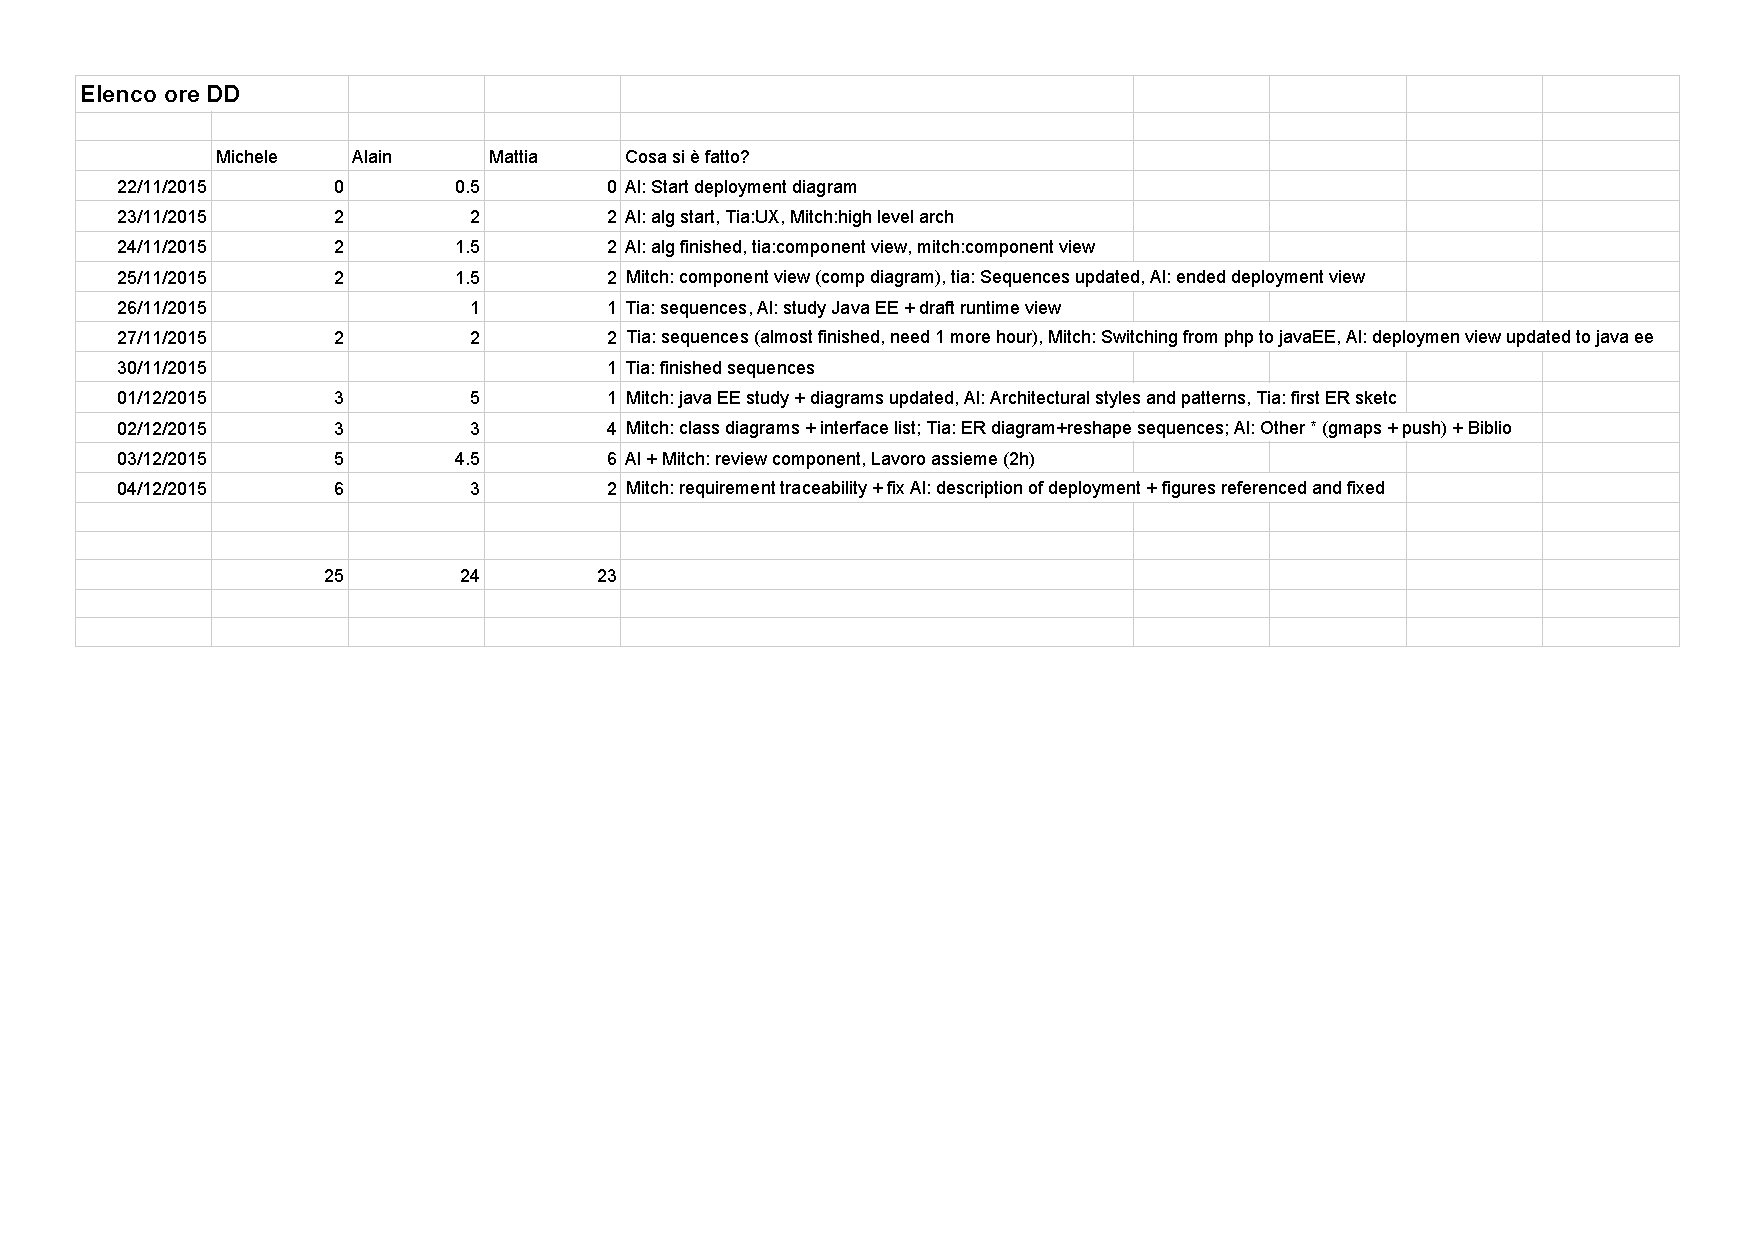
\includegraphics[width=1.2\textwidth]{img/hours.pdf}
%     \label{fig:hours}
% \end{figure}

\end{document}
